%------------------------------------------------------------------------------------
%	CHAPTER 4
%------------------------------------------------------------------------------------
\chapterimage{headerCap.jpeg}
\chapter{Lidar com Arquivos}

\begin{remark}
	Os cabelos brancos são arquivos do passado. (Edgar Alan Poe - Escritor) 
\end{remark}

\section{O Segredo}\index{Lidar com Arquivos}
Vou lhe contar um segredo, quando sai do mundo Pascal (com o Delphi) para iniciar no C (com o Java) rodei por muito tempo pois os conceitos simplesmente não se encaixavam, tinha alguns bons anos de programação mas estes não me ajudavam a migrar, foi aí que descobri um "pulo do gato", porquê não começava por algo que já sabia muito bem: manipular arquivos.

Foi exatamente os conceitos da manipulação de arquivos que me fizeram compreender a linguagem e quem sabe isso também possa lhe servir para auxiliá-lo nessa jornada com o Assembly, ou pelo menos acaba sendo bem divertido.

Primeiro devemos conhecer mais alguns valores para o registrador \textbf{EAX}, são eles:
\begin{table}[H]
	\centering 
	\begin{tabular}{c | c | l }
		\textbf{Decimal} & \textbf{Hexadecimal} & \textbf{Utilização} \\ \hline 
		3 & 0x3 & Operação de leitura do arquivo \\
		4 & 0x4 & Operação de escrita no arquivo \\
		5 & 0x5 & Operação de abertura do arquivo \\
		6 & 0x6 & Operação de fechamento do arquivo \\
		8 & 0x8 & Operação de criação do arquivo
	\end{tabular}
\end{table}

E para o registrador \textbf{ECX}:
\begin{table}[H]
	\centering 
	\begin{tabular}{c | c | l }
		\textbf{Numérico} & \textbf{Hexadecimal} & \textbf{Utilização} \\ \hline 
		0 & 0x0 & Arquivo aberto para leitura \\
		1 & 0x1 & Arquivo aberto para escrita \\
		2 & 0x2 & Arquivo aberto para leitura e escrita \\
		64 & 0x40 & Caso o arquivo não exista deve ser criado \\
		1024 & 0x400 & Preparado para novas adições de valores
	\end{tabular}
\end{table}

Sendo assim agora a nossa "bibliotecaE.inc" possui a seguinte codificação (atualize esta):
\begin{lstlisting}[]
; -------------------------------------
; Biblioteca para os registradores E
; -------------------------------------
segment .data
  LF          equ 0xA   ; Line Feed
  NULL        equ 0xD   ; Final da String
  RET_EXIT    equ 0x0   ; Operacao com Sucesso
  SYS_EXIT    equ 0x1   ; Codigo de chamada para finalizar

  STD_IN      equ 0x0   ; Entrada padrao
  STD_OUT     equ 0x1   ; Saida padrao
  STD_ERR     equ 0x2   ; Erro de operacao
 
  SYS_READ    equ 0x3   ; Operacao de Leitura
  SYS_WRITE   equ 0x4   ; Operacao de Escrita

  READ_FILE   equ 0x3   ; ler o arquivo
  WRITE_FILE  equ 0x4   ; escrever no arquivo
  OPEN_FILE   equ 0x5   ; abrir o arquivo
  CLOSE_FILE  equ 0x6   ; fechar o arquivo
  CREATE_FILE equ 0x8   ; criar o arquivo
  
  OPEN_READ   equ 0x0   ; Arquivo para leitura
  OPEN_WRITE  equ 0x1   ; Arquivo para escrita
  OPEN_RW     equ 0x2   ; Arquivo para leitura/escrita
  OPEN_CREATE equ 0x40  ; Se arquivo nao existe, cria
  OPEN_APPEND equ 0x400 ; Arquivo para adicao  

  SYS_CALL    equ 0x80  ; Envia informacao ao SO	
\end{lstlisting}	

Mas e as funções que criamos anteriormente? Essa biblioteca deve ser sempre personalizada, as funções guarde-as para quando se mostrarem necessárias, mas não neste arquivo para não colocar códigos desnecessários ao programa.

Mas acabou em comentar sobre código desnecessário para quê então constantes com o mesmo valor? (por exemplo RET\_EXIT, STD\_IN e OPEN\_READ), o motivo de criarmos essas é apenas para facilitar a leitura do código, deste modo prefiro manter assim para saber com qual operação estamos lidando.

Algo curioso acontece é com o valor de Leitura/Escrita (0x2), por exemplo, nos programas que fizemos para dar entrada no terminal utilizamos o valor 0x0 e para saída o valor 0x1, porém troque-os para 0x2 que o programa funcionará sem o menor problema\footnote{Inclusive já vi muitos tutoriais colocando esse valor como Entrada ou Saída padrão.}, porém NÃO devemos utilizá-lo, no caso da saída/entrada padrão ou estamos realizando uma leitura (através do teclado) ou uma saída (no monitor) NUNCA os dois. É uma simples questão de BOA PRÁTICA.

\section{Programa 4.1 - Ler Arquivo}\index{Lidar com Arquivos}
Devemos pensar em arquivos de modo semelhante que pensamos para o terminal, até o momento fazemos assim: \textbf{EAX} indica a operação e \textbf{EBX} para onde vai, por exemplo, 0x3 em \textbf{EAX} indica uma leitura e 0x0 em \textbf{EBX} que é na entrada padrão. Sendo assim, para um arquivo o registrador \textbf{EBX} é quem vai ditar para qual local que a informação vai entrar.

Vamos começar com a criação de um arquivo chamado "Musica.txt" com o seguinte conteúdo:
\begin{lstlisting}[]
Speak:
And disciplinary remains mercifully
Yes and um, I'm with you Derek, this star nonsense
Yes, yes
Now which is it?
I am sure of it

Music:
So, so you think you can tell
Heaven from hell?
Blue skies from pain?
Can you tell a green field
From a cold steel rail?
A smile from a veil?
Do you think you can tell?
Did they get you to trade
Your heroes for ghosts?
Hot ashes for trees?
Hot air for a cool breeze?
Cold comfort for change?
Did you exchange
A walk-on part in the war
For a leading role in a cage?
How I wish, how I wish you were here
We're just two lost souls
Swimming in a fish bowl
Year after year
Running over the same old ground
What have we found?
The same old fears
Wish you were here
\end{lstlisting}	

A música "\textit{Wish you were here}", grande sucesso da banda britânica \textit{Pink Floyd}, usaremos durante alguns programas. Faremos aqui um programa para ler esse arquivo e mostrá-lo na saída padrão. Nosso programa pode ser estruturado conforme o seguinte fluxo:
\begin{figure}[H]
	\centering
	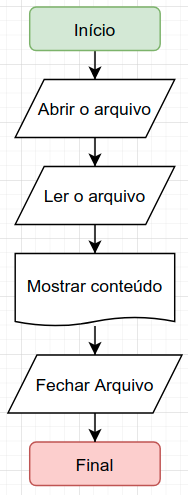
\includegraphics[width=0.2\textwidth]{Pictures/cap04/programa41}
	\caption{Fluxograma do Programa \textbf{Ler Arquivo}}
\end{figure}

O fluxo está completamente errado existe um laço de repetição para ler o arquivo, é assim que muitos vão pensar. O fluxo está correto e não existirá tal laço. Vamos para o programa que isso ficará mais claro.

Criar um arquivo chamado \textbf{lerarquivo.asm} e vamos começar com a seguinte codificação:
\begin{lstlisting}[]
%include 'bibliotecaE.inc'

SECTION .data
  nom_arq db "Musica.txt"
  tam_arq equ 1024

SECTION .bss
  fd resb 4
  buffer resb 1024
\end{lstlisting}	

Na seção \textbf{.data} temos o nome do arquivo e um tamanho em bytes deste, em Assembly precisamos saber o tamanho de tudo o que estamos fazendo, calma que existe solução para isso, esse tamanho deve conter todo o arquivo. Pode ultrapassar sem problemas, por exemplo este arquivo contém exatos 703 bytes (troque para este valor que não apresentará o menor problema).

Na seção \textbf{.bss} definimos o \textbf{fd} (abreviatura para \textit{file descriptor}) esse é o mais importante de todos pois indica o ponteiro descritor do arquivo, quando abrimos um arquivo devemos guardar seu local de memória para quando formos fazer qualquer operação com este. E temos o \textbf{buffer} que indica de quantos em quantos bytes ocorrerá um descarrego de memória.

Vamos compreender essa parte, quando lemos, ou mesmo gravamos, um arquivo esse conteúdo é lido (ou gravado) por partes e não de modo instantâneo, o SO envia a informação para um BUFFER de memória e o descarrega fisicamente na trilha de informação. Sendo assim quanto maior esse BUFFER mais rápido será feito os processos com o arquivo, esse pensamento está correto, porém mais memória será utilizada. 

Vamos iniciar a seção do programa propriamente dito:
\begin{lstlisting}[]
SECTION .text

global _start:

_start:
  mov eax, OPEN_FILE
  mov ebx, nom_arq
  mov ecx, OPEN_READ
  int SYS_CALL	
\end{lstlisting}	

Começamos com a abertura do arquivo, realizamos para isso o movimento da operação no registrador \textbf{EAX}, neste caso a abertura do arquivo, para \textbf{EBX} então recebe o nome do arquivo que tentamos abrir, \textbf{ECX} o processo que lidamos e enviamos a informação para o SO executar.

A parte mais importante é que \textbf{EAX} contém nosso \textit{File Descriptor} então antes de realizar qualquer outro processo precisamos guardá-lo:
\begin{lstlisting}[]
  mov [fd], eax	
\end{lstlisting}	

Realizamos a leitura deste:
\begin{lstlisting}[]
  mov eax, READ_FILE
  mov ebx, [fd]
  mov ecx, buffer
  mov edx, tam_arq
  int SYS_CALL	
\end{lstlisting}	

Indicamos a operação em \textbf{EAX}, o \textit{File Descriptor} com o ponteiro do arquivo para \textbf{EBX}, o tamanho do BUFFER de leitura (neste caso) em \textbf{ECX} e a quantidade de bytes que desejamos obter (por isso não existe aqui um laço de repetição) e enviamos a informação para o SO executar.

Mandamos a informação para saída padrão:
\begin{lstlisting}[]
  mov eax, SYS_WRITE
  mov ebx, STD_OUT
  mov ecx, buffer
  mov edx, tam_arq
  int SYS_CALL	
\end{lstlisting}	

Movimentos totalmente conhecidos, só que observe o seguinte, BUFFER contém TODO o conteúdo do nosso arquivo, basicamente é isso que estamos fazendo, lendo o arquivo e colocando todo seu conteúdo em BUFFER. Não tente fazer isso com arquivos "gigantes" pois provavelmente acabará com sua memória, esse programa só serve apenas para entendimento de como funciona uma leitura. Mas para frente leremos "parceladamente" um arquivo.

Precisamos fechar o arquivo:
\begin{lstlisting}[]
  mov eax, CLOSE_FILE
  mov ebx, [fd]
  int SYS_CALL	
\end{lstlisting}	

Um arquivo aberto deve ser fechado antes de finalizarmos o programa, em caso contrário este pode corromper, os movimentos são idênticos a terminar o programa. O processo em \textbf{EAX}, o \textbf{file descriptor} em \textbf{EBX} e enviamos a informação para o SO executar.

E só nos resta encerrar o programa:
\begin{lstlisting}[]
  mov eax, SYS_EXIT
  mov ebx, RET_EXIT
  int SYS_CALL	
\end{lstlisting}	

Compilamos, linkeditamos e executamos conforme visto e teremos toda a letra da belíssima música do \textit{Pink Floyd} em nosso monitor.

\section{Programa 4.2 - Gravar Arquivo}\index{Lidar com Arquivos}
Estranho como são as coisas nos Sistemas Operacionais quem conhece o MacOS ou Linux se acostuma com alguns valores em Base Octal (Octal? é uma base numérica com 8 símbolos do 0 ao 7) composta por 3 dígitos, sendo que o primeiro corresponde ao dono (criador) do arquivo, o segundo aos usuários de mesmo grupo e o terceiro a usuários externos. E esses dígitos correspondem as seguintes permissões:
\begin{itemize}[nolistsep]
	\item 1 executar
	\item 2 escrever
	\item 3 executar e escrever
	\item 4 ler
	\item 5 executar e ler
	\item 6 escrever e ler
	\item 7 executar, escrever e ler
\end{itemize}

Essas permissões devem ser definidas para cada arquivo que criamos, em linguagens de alto nível basicamente são esquecidas por um padrão definido, mas aqui são extremamente necessárias.
\\[2mm]
\begin{dica}[Na verdade]
Só precisamos decorar os valores 1, 2 e 4. Pois se pensarmos um pouco vemos que as permissões se combinam, por exemplo, o valor 3 significa a permissão 1 + 2 e assim sucessivamente.
\end{dica}

Não precisamos nos assustar pois basicamente vamos ver que tudo se trata de uma simples sequencia repetida de movimentos para os 4 registradores padrões: \textbf{EAX}, \textbf{EBX}, \textbf{ECX} e \textbf{EDX}. E garanto que tudo será bem mais simples do que se supõe.

Vamos iniciar um programa chamado \textbf{gravararquivo.asm} com a seguinte codificação:
\begin{lstlisting}[]
%include 'bibliotecaE.inc'

SECTION .data
  msg db "Hello World! Voltamos ao Inicio...", LF
  tamMsg equ $ - msg
  arq db 'Hello', NULL
  tamArq equ $ - arq
  fd dq 0
\end{lstlisting}	

Temos a mensagem (msg) que queremos gravar e seu respectivo tamanho (tamMsg). Em seguida o nome do arquivo (arq) e o tamanho desse nome (tamArq) isso é necessário para criarmos. E por fim o conhecido \textit{file descriptor} (fd) para conter o apontamento do arquivo.

\begin{lstlisting}[]
SECTION .text

global _start:

_start:
  mov eax, CREATE_FILE
  mov ebx, arq
  mov ecx, 0o664
  mov edx, tamArq
  int SYS_CALL	
\end{lstlisting}	

Primeiro passo é mover o valor 0x8 para \textbf{EAX} que indica um processo de criação (ou abertura se o arquivo existe), em seguida o nome deste para \textbf{EBX}, em \textbf{ECX} colocamos o valor \textbf{0o664} os dois primeiros indicam que se trata de um valor na base octal e esses são: 6 (permissão de escrever e ler para o dono), 6 (permissão de escrever e ler para os usuários do mesmo grupo) e 4 (permissão de ler para qualquer outro tipo de usuário), colocamos o tamanho do nome do arquivo em \textbf{EDX} e por fim dizemos ao SO para executar essa ação.

\begin{lstlisting}[]
  mov [fd], eax  
  mov eax, WRITE_FILE
  mov ebx, [fd]
  mov ecx, msg
  mov edx, tamMsg
  int SYS_CALL	
\end{lstlisting}	

Para executar a ação de gravar em bem semelhante ao que já vimos na saída padrão com a ~diferença que em \textbf{EBX} deve ir o apontamento para \textit{file descritor}.

\begin{lstlisting}[]
  mov eax, CLOSE_FILE
  mov ebx, [fd]
  int SYS_CALL	
\end{lstlisting}	

Fechamos o arquivo, aqui este comando se torna essencial pois caso contrário com certeza iremos corrompê-lo.

\begin{lstlisting}[]
  mov eax, SYS_EXIT
  mov ebx, RET_EXIT
  int SYS_CALL	
\end{lstlisting}	

E só nos resta avisar ao SO que terminamos o programa. Porém vamos alguns detalhes que ainda devemos compreender. Compilamos, linkeditamos e executamos o programa e teremos um arquivo chamado \textbf{Hello} criado e ao abri-lo existe uma linha com o valor de \textbf{msg}. Executamos novamente e continua com uma única linha. Abrimos com um editor qualquer alteramos essa linha completamente e inclusive colocamos mais linhas e ao executarmos novamente o arquivo retorna para a uma única linha original. Mas qual o motivo disso acontecer?

Quando abrimos um arquivo estamos posicionados na linha 0 e coluna 0 deste, sendo assim sempre o estamos iniciando. Mas porquê perde o conteúdo que escrevemos? Pois esse é o objetivo do 0x8 dizer que queremos um arquivo novo em folha, o que é bem diferente do 0x5 que vimos no programa anterior.

Mas como fazemos então para criar ou abrir um arquivo se esse já existe e principalmente colocar mais conteúdo? Isso deixaremos para responder no próximo programa.

\section{Programa 4.3 - Adicionar no Arquivo}\index{Lidar com Arquivos}
Conseguimos então criar um arquivo e adicionar conteúdo neste, porém toda vez que rodamos o programa todo arquivo é apagado e não conseguimos manter o conteúdo anterior.

Para resolver este problema criamos um novo arquivo chamado "maisUma.asm" e adicionamos o seguinte conteúdo (coloque o arquivo "Hello" criado no programa anterior nesta pasta):
\begin{lstlisting}[]
%include 'bibliotecaE.inc'

SECTION .data
  msg2    db "Aqui temos mais uma linha", LF
  tamMsg2 equ $ - msg2
  arq     db 'Hello'
  tamArq  equ $ - arq
  fd      dq 0 ;
\end{lstlisting}

Na nossa seção de constantes temos a mensagem que desejamos adicionar no arquivo: "Aqui temos mais uma linha", o nome do arquivo e nosso já conhecido ponteiro (\textit{File Descriptor}) para o arquivo.

Todo "pulo do gato" esta no próximo código do programa:
\begin{lstlisting}[]
SECTION .text

global _start:

_start:
  mov eax, OPEN_FILE
  mov ebx, arq
  mov ecx, OPEN_CREATE+OPEN_WRITE+OPEN_APPEND
  mov edx, 0o664
  int SYS_CALL
  
  mov [fd], eax	
\end{lstlisting}	

Movimentamos para \textbf{EAX} o código de abertura do arquivo e para \textbf{EBX} o nome deste, porém para \textbf{ECX} realizamos uma combinação de 3 valores:
\begin{itemize}[nolistsep]
	\item \textbf{OPEN\_CREATE} (0x40) - Se o arquivo não existe cria.
	\item \textbf{OPEN\_WRITE} (0x4) - Abrir o arquivo para escrita.
	\item \textbf{OPEN\_APPEND} (0x400) - Abrir o arquivo de modo inclusão.
\end{itemize}	

É exatamente essa combinação que permite Criar/Abrir o arquivo em modo para adição de conteúdo, em \textbf{EDX} colocamos as permissões do arquivo e enviamos ao SO proceder essas instruções, para \textbf{EDX} indicamos as permissões do arquivo conforme já vimos.

\begin{lstlisting}[]
escreverNoArquivo:
  mov eax, WRITE_FILE
  mov ebx, [fd]
  mov ecx, msg2
  mov edx, tamMsg2
  int SYS_CALL 	
\end{lstlisting}	

Se fizermos um comparativo com o programa anterior teremos aqui os mesmos movimentos para gravar a informação no arquivo porém como este foi aberto com o parâmetro de adição toda essa informação será inserida ao final do conteúdo da última linha no arquivo.

\begin{lstlisting}[]
fecharArquivo:
  mov eax, CLOSE_FILE
  mov ebx, [fd]
  int SYS_CALL    

final:
  mov eax, SYS_EXIT
  mov ebx, EXIT_SUCESS
  int SYS_CALL 	
\end{lstlisting}	

E fazemos os movimentos para fechar o arquivo e encerrar o programa. Sabemos porém que o mais interessante a cada vez que rodamos este programa uma nova linha será adicionada ao arquivo. Então se pararmos para pensar até este ponto já sabemos ler um arquivo, iniciar, gravar uma informação em um novo e adicionar mais conteúdo.

\section{Programa 4.4 - Localizar no Arquivo}\index{Lidar com Arquivos}
Talvez uma das partes mais complicada seja localizar um determinado ponto dentro do arquivo, permita-me reformular esta frase, já vamos ter que aprender mais valores e adicionar mais informação a nossa biblioteca.

Primeiro devemos conhecer mais alguns valores para o registrador \textbf{EAX}, são eles:
\begin{table}[H]
	\centering 
	\begin{tabular}{c | c | l }
		\textbf{Decimal} & \textbf{Hexadecimal} & \textbf{Utilização} \\ \hline 
		18 & 0x13 & Operação de localização no arquivo
	\end{tabular}
\end{table}

E para o registrador \textbf{EDX}:
\begin{table}[H]
	\centering 
	\begin{tabular}{c | c | l }
		\textbf{Decimal} & \textbf{Hexadecimal} & \textbf{Utilização} \\ \hline 
		0 & 0x0 & A partir do início do arquivo \\
		1 & 0x1 & Na posição que estiver o cursor \\
		2 & 0x2 & Final do Arquivo
	\end{tabular}
\end{table}

Sendo assim agora a nossa "bibliotecaE.inc" possui a seguinte codificação complementar (atualize esta):
\begin{lstlisting}[]
; -------------------------------------
; Biblioteca para os registradores E
; -------------------------------------
segment .data
...
SEEK_FILE   equ 0x13  ; posicionar no arquivo
SEEK_SET    equ 0x0   ; inicio do arquivo
SEEK_CUR    equ 0x1   ; posicao do cursor
SEEK_END    equ 0x2   ; final do arquivo	
\end{lstlisting}	

Vamos com calma para se posicionar em um arquivo, após abrí-lo precisamos em \textbf{EAX} indicar a operação, ou seja, o SEEK\_FILE (0x19), para \textbf{EBX} nosso já conhecido \textit{File Descriptor} (ponteiro do arquivo), em \textbf{ECX} a quantidade de caracteres para saltar (essa é a parte complicada) e finalmente em \textbf{EDX} se desejamos proceder o salto a partir do início no arquivo (SEEK\_SET), ou do ponto de leitura que já estamos (SEEK\_CUR - obviamente no momento que abrimos o arquivo esse valor será idêntico ao primeiro) ou estamos lendo de trás para frente a partir do final no arquivo (SEEK\_END).

Lembra da nossa música que lemos no primeiro programa dessa seção? Então coloque-a nesta pasta além do makefile, e vamos criar um novo arquivo chamado "lerPosicao.asm" com a seguinte codificação inicial:

\begin{lstlisting}[]
%include 'bibliotecaE.inc'

SECTION .data
  arq    db "Musica.txt"
  tam    equ 1024

SECTION .bss
  fd     resb 4
  buffer resb 1024

SECTION .text

global _start:

_start:
  mov eax, OPEN_FILE
  mov ebx, arq
  mov ecx, OPEN_READ
  int SYS_CALL
  mov [fd], eax
\end{lstlisting}	

Se ainda tem alguma dúvida sobre qualquer código escrito até aqui recomendo que retorne ao início deste capítulo e reveja qualquer conceito, pois neste ponto vamos nos concentrar apenas na parte de pegar uma determinada informação e ler.

Vamos criar três blocos:
\begin{lstlisting}[]
posicionar:
  ; TODA PESQUISA VEM AQUI

ler:
  mov eax, READ_FILE
  mov ebx, [fd]
  mov ecx, buffer
  mov edx, tam
  int SYS_CALL

saidaNoConsole:
  mov eax, SYS_WRITE
  mov ebx, STDOUT
  mov ecx, buffer
  mov edx, tam
  int SYS_CALL
\end{lstlisting}	

Calma que está faltando informação, o bloco \textbf{ler} e \textbf{saidaNoConsole} fazem exatamente a mesma coisa que vimos no primeiro programa. E os dois últimos blocos:
\begin{lstlisting}[]
fechar:
  mov eax, CLOSE_FILE
  mov ebx, [fd]
  int SYS_CALL

termino:
  mov eax, SYS_EXIT
  mov ebx, EXIT_SUCESS
  int SYS_CALL
\end{lstlisting}

Também já estamos cansados de ver neste capítulo procedendo o fechamento do arquivo e o término do programa.

\subsection{Concentrar na Pesquisa}\index{Lidar com Arquivos}
Vamos nos concentrar exclusivamente naquele bloco posicionar, se executarmos da forma como se encontra o código temos exatamente o primeiro programa encontrado neste capítulo, ou seja, vamos ler o arquivo inteiro, mas se adicionarmos a seguinte codificação:
\begin{lstlisting}[]
posicionar:
  mov eax, SEEK_FILE
  mov ebx, [fd]
  mov ecx, 144
  mov edx, SEEK_SET
  int SYS_CALL
\end{lstlisting}

Começaremos a ler o nosso arquivo a partir do caractere 144, se contar essa posição no arquivo teremos bem no começo da música e saltamos toda a parte da introdução, ou seja mostra a partir de: \\
{\ttfamily So, so you think you can tell... Wish you were here}

O mesmo efeito teria o valor de SEEK\_CUR em \textbf{EDX} pois como acabamos de abrir o arquivo, sua posição inicial de leitura é 0 e contaremos os mesmos 144 caracteres a partir dessa posição, porém se mudamos para:

\begin{lstlisting}[]
posicionar:
  mov eax, SEEK_FILE
  mov ebx, [fd]
  mov ecx, 144
  mov edx, SEEK_SET
  int SYS_CALL

  mov eax, SEEK_FILE
  mov ebx, [fd]
  mov ecx, 428
  mov edx, SEEK_CUR
  int SYS_CALL
\end{lstlisting}

No primeiro conjunto estamos indo até a posição 144 (ou seja no começo da música propriamente dito), em seguida percorremos mais 428 caracteres e temos basicamente o último verso desta a partir de: \\
{\ttfamily Swimming in a fish bowl... Wish you were here}

Também podemos nos posicionar de trás para frente:
\begin{lstlisting}[]
posicionar:
  mov eax, SEEK_FILE
  mov ebx, [fd]
  mov ecx, -131
  mov edx, SEEK_END
  int SYS_CALL
\end{lstlisting}

E obtermos exatamente o mesmo resultado. Calma que este programa é apenas para exemplificar como é aplicado os saltos dentro de arquivos e na prática não faríamos desta forma, provavelmente pedimos a informação para o usuário (como uma palavra dentro do arquivo) e damos saltos até localizá-la.

% Final do Capítulo
\clearpage